\documentclass[../report.tex]{subfiles}
\graphicspath{{\subfix{../image/}}}

\begin{document}
\subsection{Forklifts}

\begin{wrapfigure}{r}{0.5\textwidth}
    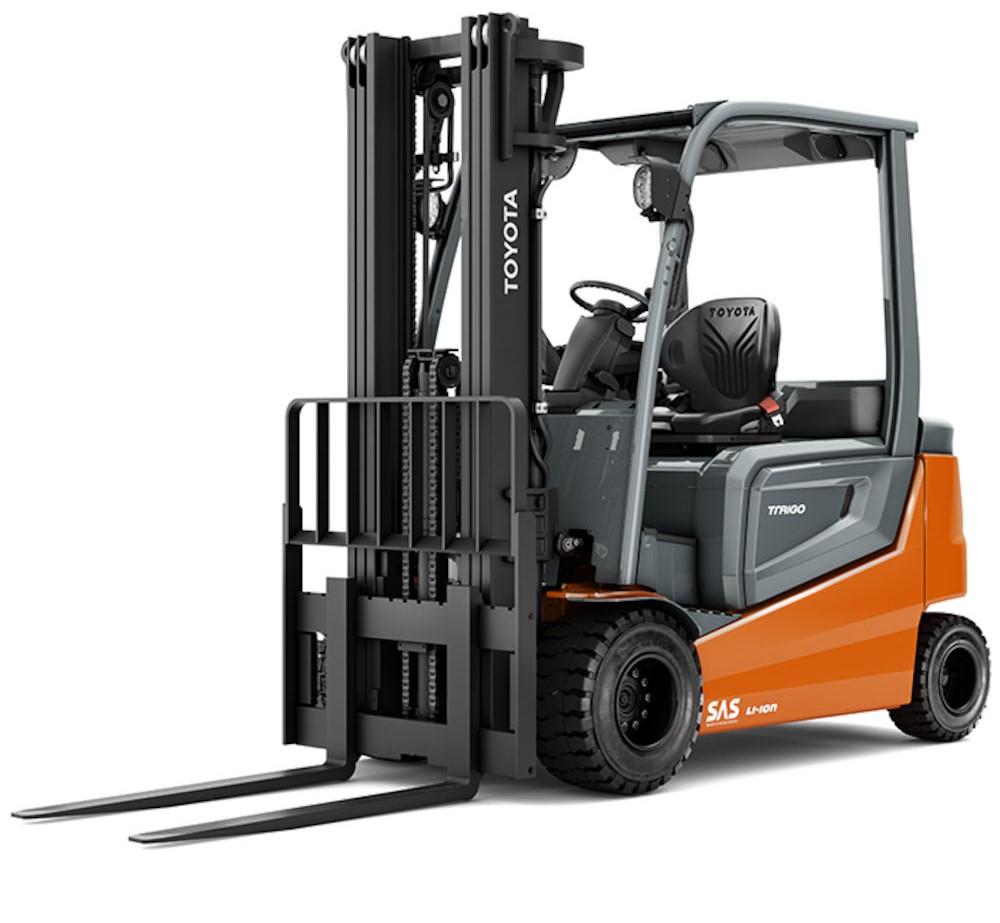
\includegraphics[width=0.35\textwidth]{../image/baltic.toyota-forklifts.jpeg}
    \caption{Counterbalanced Forklift}
    \label{fig:forklift}
\end{wrapfigure}
When looking into forklifts there are different types, that are task dependent.
Some of those are the pallet jack or Low Lift Truck, Stacker and the most common Counterbalanced forklift.

The basic parts of the Counterbalanced forklift as seen in the picture.
\begin{center}
    \begin{enumerate}
    \item fork
    \item mast
    \graphicspath{{\subfix{../image/}}}
    \item drive and steering wheels 
    \item counterweight
    \item motor compartment
    \end{enumerate}
\end{center}

\subsubsection{Functionality}
For the functionality of forklifts there are two different subjects that concern us.
For one the drive, which should make it possible to rotate 360° around the center axle
and the lifting of the fork it self.
The amount of lifting is dependent on the type of forklift. Therefore the task of a low lift 
truck is lifting of the ground for simple 2 dimensional movement and other types need
to be able to lift up to multiple pallets or meters, where also the name stacker derives from.

\textbf{Lifting}
The lifting mechanism works by actuating an actuator which is and hydraulic cylinder in this 
case. A chain that is connected between an anchor, roller and the fork lifts the fork and by 
making use of the leverage of this system the forklift can lift greater weights than when 
connecting the fork directly to the actuator.

\textbf{Driving}
On a forklift as seen in [\ref{fig:forklift}], the front wheels are connected to the drive
while the back wheels are able to rotate 360° and only act for steering.



\end{document}